\documentclass{projdoc}

\title{Software Design}

\begin{document}
\tablestables
\newpage

\section{Introduction}

This document outlines the design and development process of the cr\^epe game engine,
detailing the key decisions made during its creation. The primary goal of this engine
is to offer a streamlined, Unity-like experience tailored for developing 2D games
similar to Jetpack Joyride.

The cr\^epe engine is designed to ease the transition for developers familiar with
Unity, ensuring minimal friction when switching platforms. Our aim is to preserve
many of Unity’s core features while introducing a lightweight and open-source
alternative, licensed under the MIT License.

The engine is primarily aimed at indie developers who have prior experience with
Unity and are looking for a flexible, cost-effective solution with familiar
workflows.

\section{Overview}
As described above, the cr\^epe game engine's goal is to offer a Unity-like experience
tailored for developing 2D games similar to Jetpack Joyride. That is why Jetpack
Joyride and Unity provided the main inputs for this game engine design. Firstly, a
quick overview will be given of the Unity game engine, in particular the \gls{ecs}.
Secondly, this Overview will quickly talk you through some of the most important
parts of the game engine, and why these parts are needed to create the Jetpack
Joyride game.

\subsection{ECS}
The Unity game engine is structured using the Entity Component System (\gls{ecs})
(as shown in \cref{fig:ECS Block Diagram}). The \gls{ecs} is made out of three
main subsystems, namely entities, components and systems. Entities are just IDs.
An entity is also called a GameObject in Unity and it is made out of one (or
more) components. Components are the classes that hold the data. The components
determine what kind of entity it is (e.g. an enemy, audio, and so on). Systems take
care of the behavior of the entities. Systems mainly read and write the enity's
components data. The \gls{ecs} clearly distinguishes the data (components) from the
functionality (systems).

\begin{figure}
	\centering
	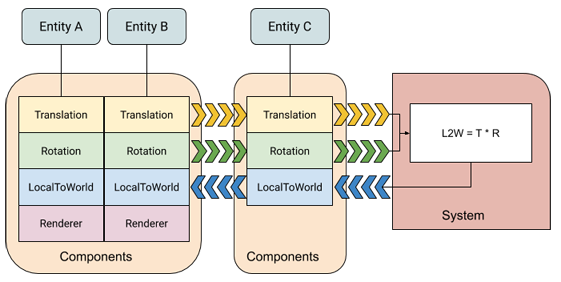
\includegraphics[width=0.5\textwidth]{img/ECSBlockDiagram.png}
	\caption{ECS design pattern}
	Source: \autocite{img:ECSBlockDiagram}
	\label{fig:ECS Block Diagram}
\end{figure}

The \gls{ecs} will also be used at the cr\^epe game engine. Everything (from the
protagonist and bullets to the walls and enemies) in the cr\^epe game engine will
be a GameObject (a.k.a. entity). The game programmer must program his game by
creating all kind of GameObjects and placing them in one (or multiple) scenes, just
like Unity.

\subsection{Jetpack Joyride}
Firstly, some background information about Jetpack Joyride. Jetpack Joyride is a
side-scrolling endless runner action video game created by Halfbrick Studios. The
protagonist is called Barry Steakfries, who the player controls as he steals a
bullet-powered jet pack from a top-secret laboratory \autocite{wiki:JetpackJoyride}.
A screenshot from the game can be seen in \cref{fig:JetpackJoyride} (pleae be
aware that the goal of this project is not to create an exact replica of Jetpack
Joyride, it is only used as a source of inspiration).

\begin{figure}
	\centering
	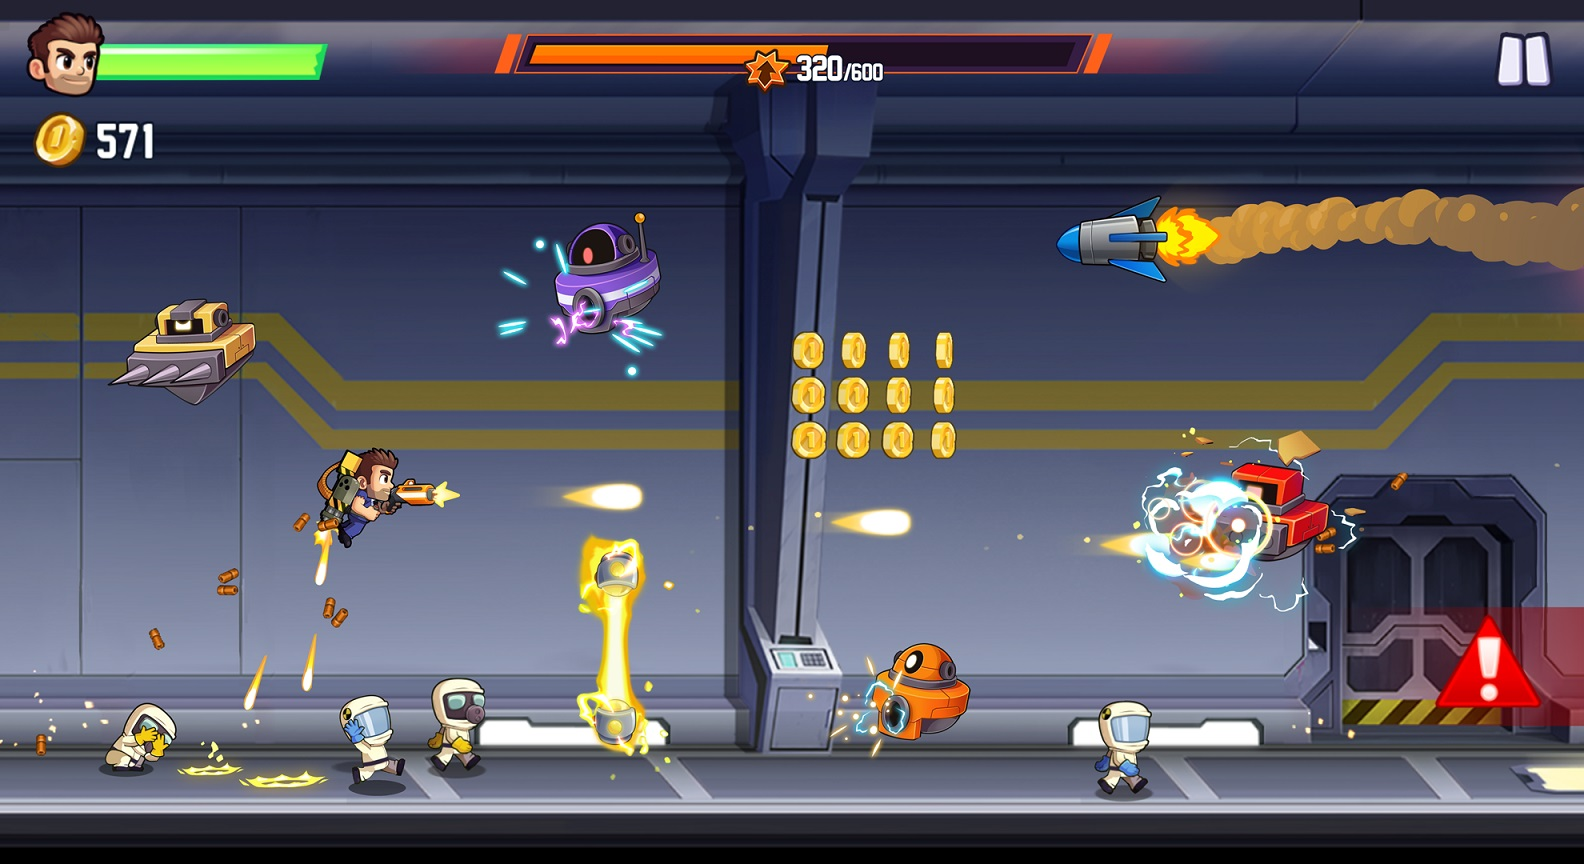
\includegraphics[width=0.5\textwidth]{img/JetpackJoyride.jpg}
	\caption{Jetpack Joyride}
	Source: \autocite{img:JetpackJoyride}
	\label{fig:JetpackJoyride}
\end{figure}

The protagonist wears a jetpack with which he can float in the air. The player must
avoide obstacles (such as lasers, missiles and zappers) by floating at the right
height. The player can control the protagonist's jetpack, thereby also controlling
the protagonist's height. The protagonist experiences gravity and other forces (like
the force from his jetpack pushing him upwards). These forces should be easily
programmable by the game programmer. That is why a physics system is needed in the
cr\^epe game engine. Only very limited/easy physics are needed for Jetpack Joyride,
that is why this is only supported by the cr\^epe game engine.

The protagonist must avoid obstacles. That is why the cr\^epe game engine should
also support a collision system. Again, only very limited/easy collision is needed
for Jetpack Joyride, that is why only very limited/easy collision is supported
by the cr\^epe game engine.

The game must, of course, also be visible to and playable by the user. A rendering
system will take care of rendering (displaying) the game and its GameObjects. An
input system will take care of all the inputs (mouse and keyboard).

Jetpack Joyride also offers audio. A system will take care of the audio in the cr\^epe
game engine.

Particles are very common in Jetpack Joyride, e.g. underneath the jetpack and behind
the rockets. Particles will be supported by the particle system.

The start of a scene is described in a scene. However, the game programmer might also
want to write game logic code which is running during the game (e.g. to switch to a
new scene or to perform a custom action at a collision). For these purposes, Unity
uses scripts. These scripts will also be supported by the cr\^epe game engine.

Finally, as an extra, replay functionality will be supported by the cr\^epe game
engine. A dedicated replay system will be used to support replay.

It turns out that a physics, collision, rendering, input, audio, particle, script,
and replay system are needed to create the Jetpack Joyride game. These systems form
the main part of the \gls{ecs}. The design of these eight systems in combination with
\gls{ecs}, will be briefly discussed in the next parts of this design document.

\section{Design}

\subsection{Rendering}

\subsection{Physics}

\subsection{Scripting}

The scripting interface was designed around a `target' \gls{api} (described by
\cref{req:script:interface,req:script:user-class,req:script:direct-instance,req:script:direct-run}).
An example of this \gls{api} is shown below:\noparbreak

\begin{blockcode}
class MyScript : public BehaviorScript {
	void update() {
		// update code here
	}
	// init() also exists, but is empty by default
};

{ // in scene initialization
	GameObject & obj = ...;
	obj.add_component<MyScript>();
}
\end{blockcode}

The above call to \codeinline{GameObject::add_component} cannot work correctly
without significantly increasing the complexity of the component manager, so the
following restrictions were taken into account when creating the script system
architecture:\noparbreak

\begin{itemize}
	\item The first template parameter passed to \codeinline{GameObject::add_component}
		\emph{must} be a base `script \emph{component}' class, so each derived user
		script class is instantiated in the same generic script list.
	\item C++ does not allow passing types (i.e.~\codeinline{MyScript} in this case) as
		function parameters, so a function call like
		\codeinline{add_component<BehaviorScript>(MyScript)} cannot be realized.
\end{itemize}

\subsubsection{Architecture}

The restrictions detailed at the start of this section are mitigated as
follows:\noparbreak

\begin{itemize}
	\item User scripts are split into two classes---
		\begin{enumerate}
			\item a script \emph{interface} class (\codeinline{Script})
			\item a script \emph{component} class (\codeinline{BehaviorScript})
		\end{enumerate}
	\item \codeinline{GameObject::add_component} receives the script \emph{component}
		as template parameter
	\item \codeinline{GameObject::add_component} now always returns a reference to the
		component instance
	\item The script component class has a setter function that takes a template
		parameter for classes derived from the base script \emph{interface} class
\end{itemize}

\Cref{fig:class-scripts} shows the resulting structure as a class diagram. It
contains the following classes:\noparbreak
\begin{description}
	\item[Script] This is the script \emph{interface}, and is used by the game
		programmer to create derived script classes. All methods in this class are
		declared virtual and have an empty implementation.

		This class' methods are protected by default, and a friend relation to
		\codeinline{ScriptSystem} is used to ensure only \codeinline{ScriptSystem} is
		able to call these methods.

		Only classes derived from \codeinline{Script} can be used with
		\codeinline{BehaviorScript::set_script}'s template parameter \codeinline{T}. This
		function returns a reference to the \codeinline{BehaviorScript} instance it was
		called on so it can be chained after the call to
		\codeinline{GameObject::add_component}.
	\item[BehaviorScript]
		This is the script \emph{component}, and is given as the template parameter to
		\codeinline{GameObject::add_component}.

		This class also uses a friend relation to \codeinline{ScriptSystem} to restrict
		access to its private reference member \codeinline{script}.
	\item[ScriptSystem] This is the system class that runs the methods implemented in
		the derivative instances of \codeinline{Script}.
\end{description}

\begin{figure}
	\centering
	\includepumldiag{img/class-scripts.puml}
	\caption{User script class diagram}
	\label{fig:class-scripts}
\end{figure}

\subsection{Audio}

Since writing a custom real-time audio mixing engine is outside the scope of this
project\mref and C++ does not provide a built-in cross-platform audio \gls{api}, the
audio system inside the cr\^epe engine is implemented as a fa\c{c}ade around an
existing audio library.

\subsubsection{Libraries}
\label{sec:audio:libs}

This subsection compares various standalone audio libraries for suitability. After
searching for libraries (search terms: `dynamic/adaptive audio', `real-time audio',
`audio library', `game audio engine'), several libraries were found. These libraries
were checked against the audio engine requirements \autocite{crepe:requirements} and
then tested by writing the same benchmark-style \gls{poc} using the remaining
qualifying libraries:\noparbreak
\begin{enumerate}
	\item Load a background track (Ogg Vorbis)
	\item Load three short samples (WAV)
	\item Start the background track
	\item Play each sample sequentially while pausing and resuming the background track
	\item Play all samples simultaniously
	\item Stop all audio and exit
\end{enumerate}

Of these libraries the following were determined to be unsuitable for use in this
project:\noparbreak
\begin{description}
	\item[FMOD \autocite{lib:fmod}] Is proprietary (violates \cref{req:lib:license}).
	\item[PortAudio \autocite{lib:portaudio}] Does not handle mixing.
	\item[miniaudio \autocite{lib:miniaudio}] Tested by implementing a \gls{poc}, but
		dropped due to very limited codec support (WAV, MP3 and FLAC only); Also does not
		have an \gls{api} reference (only programming manual).
	\item[YSE \autocite{lib:yse}] Attempted to write \gls{poc}, but CMake configuration
		in repository is broken; This project seems to have been abandoned.
\end{description}

The only library that remained after these tests is SoLoud \autocite{lib:soloud}. It
is Zlib/LibPng licensed and provides a high-level object-oriented C++ \gls{api}.
\Cref{sec:audio:architecture} describes the fa\c{c}ade written for this library.

\subsubsection{Architecture}
\label{sec:audio:architecture}

\Cref{fig:class-audio-facade} shows a class diagram of the audio fa\c{c}ade. It
contains the following classes:
\begin{description}
	\item[SoundContext] This is a wrapper around the \codeinline{SoLoud::soloud}
		`engine' class, and is therefore implemented as a singleton. This ensures the
		audio engine is initialized before \codeinline{Sound} is able to use it.

		This class is friends with \codeinline{Sound}, so only \codeinline{Sound} is able
		to get the \codeinline{SoundContext} instance.
	\item[Sound] This is a wrapper around the \codeinline{SoLoud::Wav} class, and uses
		cr\^epe's \codeinline{Asset} class to load an audio sample instead.
\end{description}

\begin{figure}
	\centering
	\includepumldiag{img/facade-audio.puml}
	\caption{Audio fa\c{c}ade class diagram}
	\label{fig:class-audio-facade}
\end{figure}

\subsection{Input}

\subsection{Physics}

\section{Tools}

\section{Conclusion}

\end{document}

